\begin{tikzpicture}[font=\footnotesize]
\node (A) at (0,0) [minimum size=1cm] {}; \Alice{0}{0}{0.4};
\node (B) [right of = A, node distance = 4cm, minimum size=1cm] {}; \Bob{4cm}{0}{0.4};
\node (0a) [below of=A, node distance=0.7cm] {};
\node (0b) [below of=B, node distance=0.7cm] {};
\draw[latex-latex] (0a) -- (0b) node [midway,above] {random $k,s > 3$} node [midway,below] {$ks \equiv e \pmod N$};
\node (1a) [below of=0a, node distance=0.5cm] {};
\node (1b) [below of=0b, node distance=0.5cm] {};
%\draw[-latex] (1a) -- (1b) node [midway,above] {};
\node (2a) [below of=1a, node distance=0.5cm] {};
\node (2b) [below of=1b, node distance=0.5cm] {};
\draw[latex-latex] (2b) -- (2a) node [midway,above] {random $c$};
\node (3a) [below of=2a, node distance=0.5cm] {$m = c^d $};
\node (3b) [below of=2b, node distance=0.5cm] {};
%\draw[-latex] (3a) -- (3b) node [midway,above] {};
\node (4a) [below of=3a, node distance=0.5cm] {$x = m^k $};
\node (4b) [below of=3b, node distance=0.5cm] {};
\draw[-latex] (4a) -- (4b) node [midway,above] {};
\node (5b) [below of=4b, node distance=0.5cm] {$x^s \overset{?}{=} c$};
\end{tikzpicture}
